\documentclass{article}
\usepackage[utf8]{inputenc}
\usepackage[margin=1in]{geometry}
\usepackage{siunitx}
\usepackage[autocite=superscript,backend=biber,sorting=none]{biblatex} % if lag: change biber to bibtex, recompile, the change back to biber and should be good!

\usepackage{hyperref}
\usepackage[noabbrev]{cleveref}
\usepackage{graphicx}
\usepackage{float}
\usepackage{pdflscape}
\usepackage{pdfpages}
\usepackage{titlepic}

\title{Braphy}
\author{Alice Deimante Neimantaite \\ Lisa Sjöblom \\ Daniel Westerlund}
\date{June 2020}
\titlepic{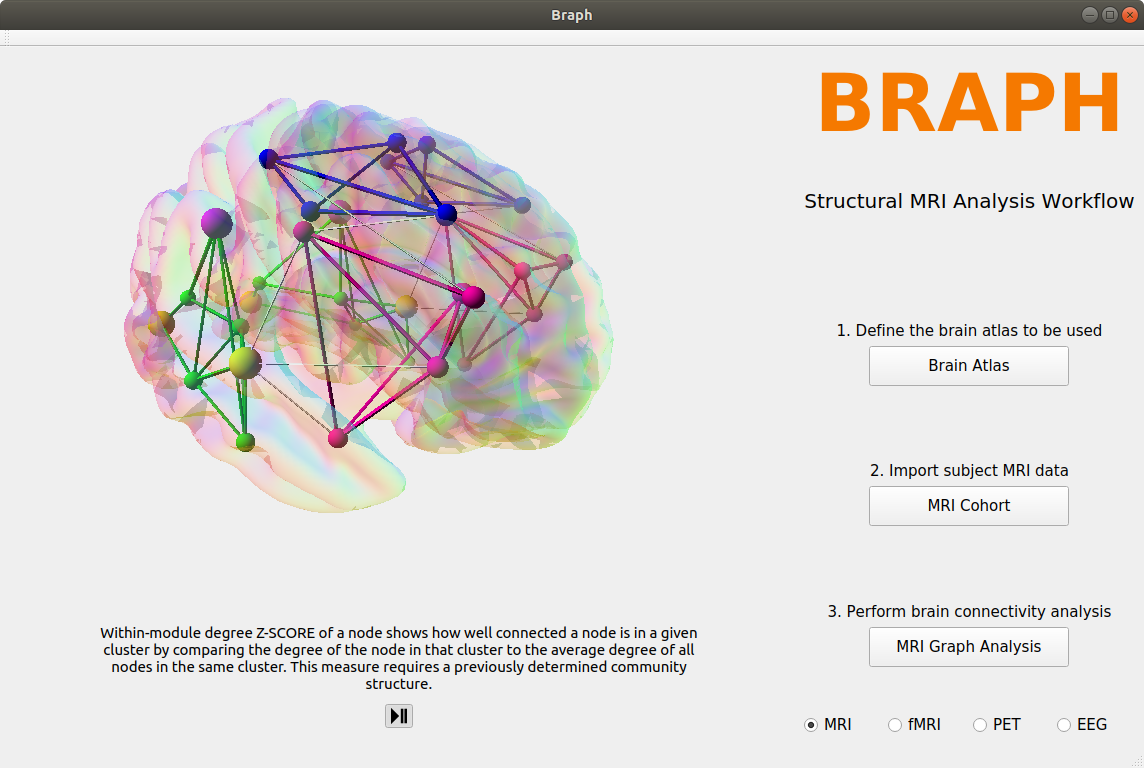
\includegraphics[width=\textwidth]{front_page.png}}

\begin{document}

\maketitle
\clearpage

\section{Introduction}

This document describes the current state of the python version of Braph 2.0, or as we call it, Braphy. We focus on describing the parts that differ from Braph 1.0, and will therefore assume that the reader has previous knowledge about this software. In the future, our idea is that this document can be developed into a full manual of Braphy.

We have tried to finish the implementation for MRI and fMRI first, and have left the other data formats for the future. Hence, these are the only ones described here.


\section{MRI}

\subsection{Graph Analysis MRI}


\begin{figure}[h]
    \centering
    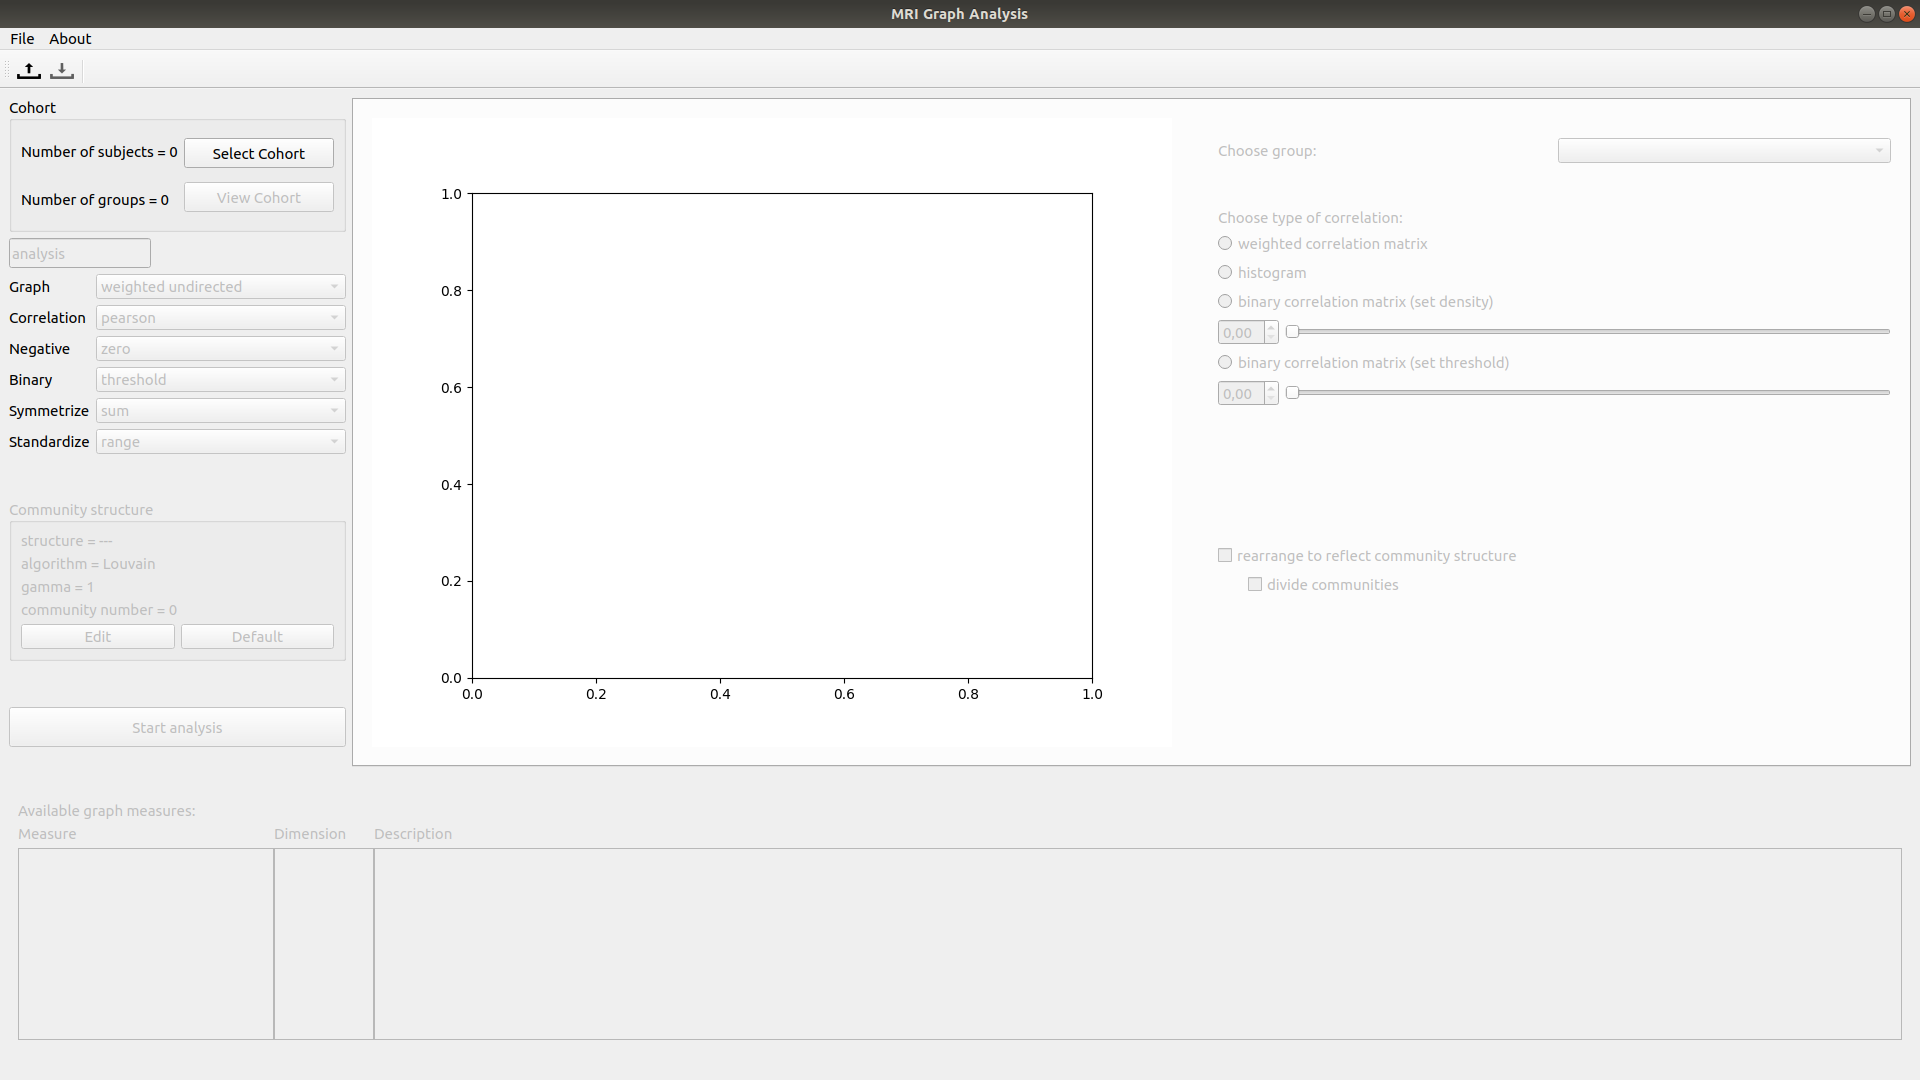
\includegraphics[width=\linewidth]{graph_analysis_locked.png}
    \caption{The initial view in the graph analysis module.}
    \label{fig:locked}
\end{figure}

\begin{figure}[h]
    \centering
    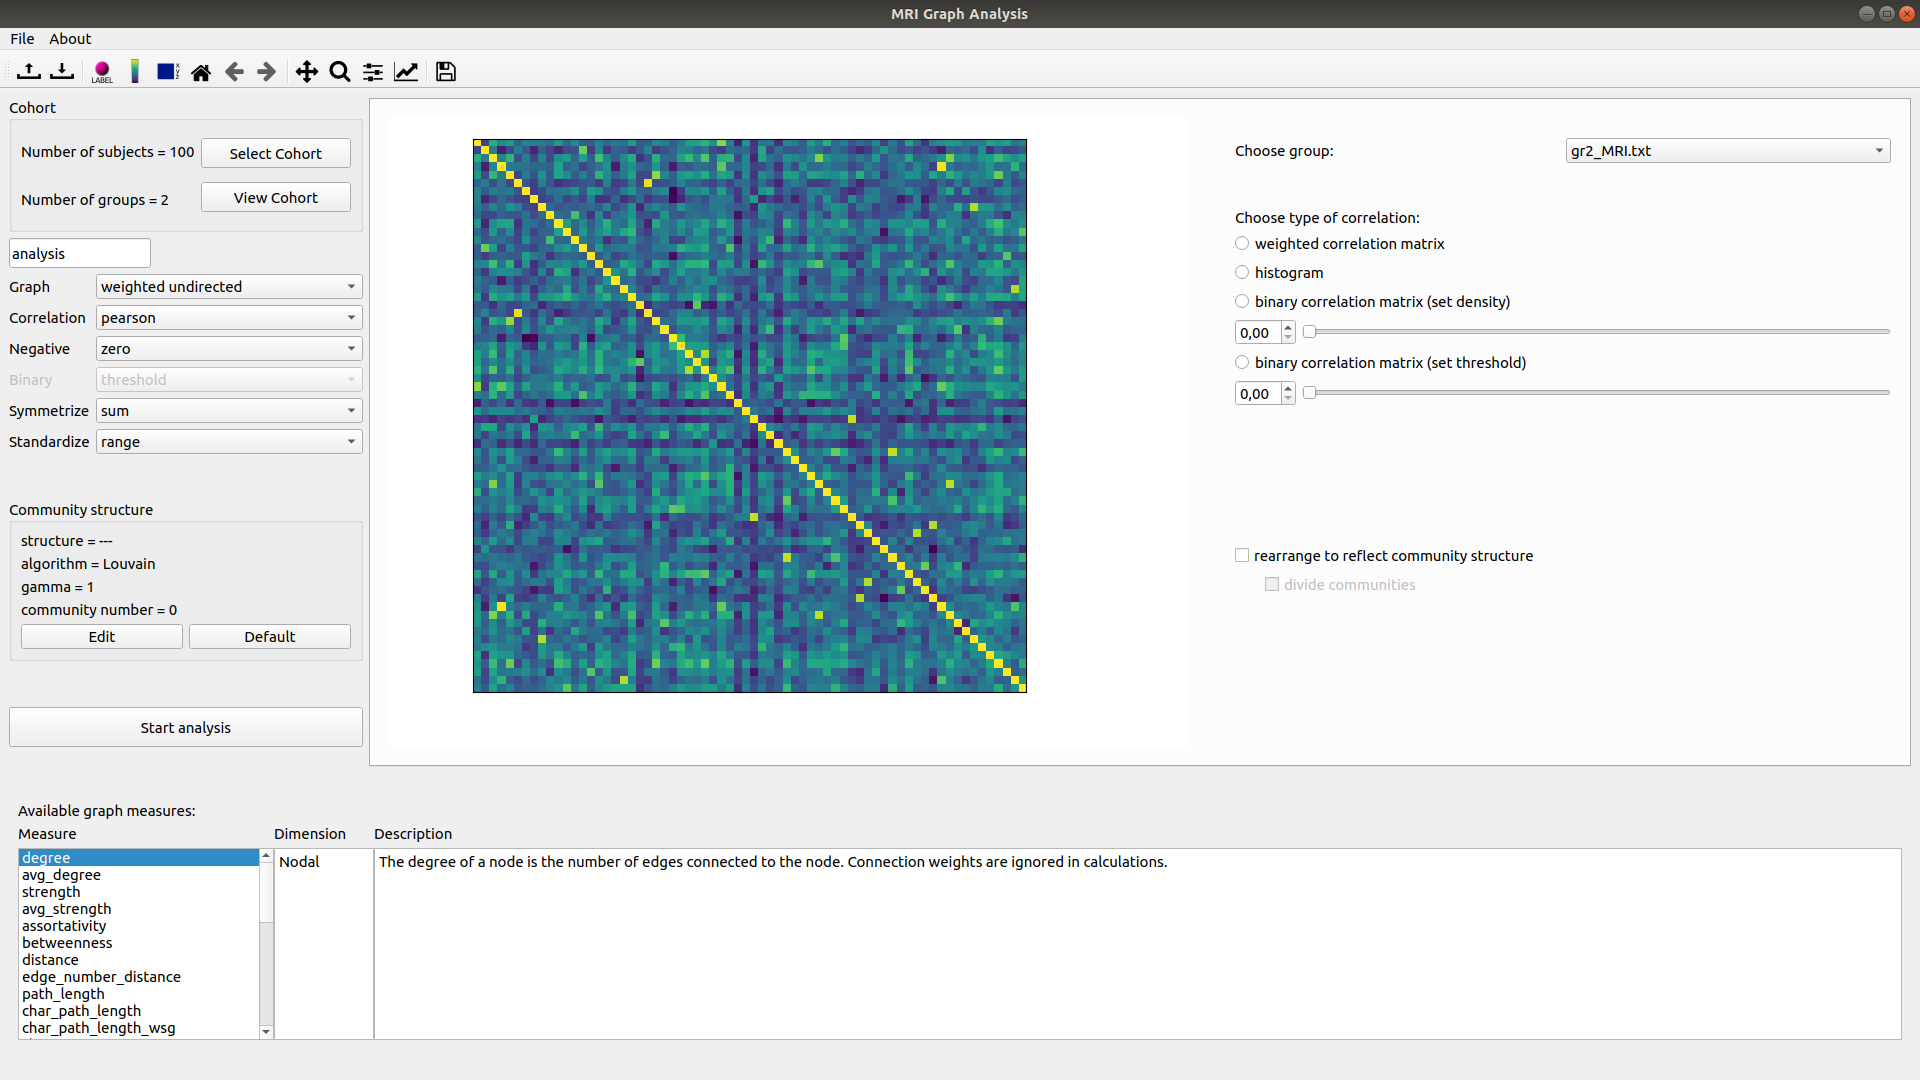
\includegraphics[width=\linewidth]{graph_analysis_cohort.png}
    \caption{The graph analysis GUI after a cohort has been loaded.}
    \label{fig:started}
\end{figure}

When the MRI Graph Analysis GUI is opened, the only action available is to load a cohort or an analysis, see \cref{fig:locked}. If you select and load a .cohort file, more options will be enabled, see \cref{fig:started}. In our version we have added the 'View Cohort' button, so that you can select a new cohort if you change your mind.

As you can see to the left in \cref{fig:started}, we have added the ability to change several graph settings. Only settings relevant for the current graph type are enabled. Further down, the 'Subgraph analysis' button has been removed. This button is instead added to the community structure window, which will be discussed later. At the bottom of the window, the measure table can be seen. Only the description of the selected measure is displayed, to avoid clutter. 

The toolbar is located at the top of the window. The first two icons correspond to opening and saving the analysis. Next, there is a set of buttons that lets the user alter the correlation matrix plot.

\subsubsection{Community Structure GUI}

\begin{figure}[h]
    \centering
    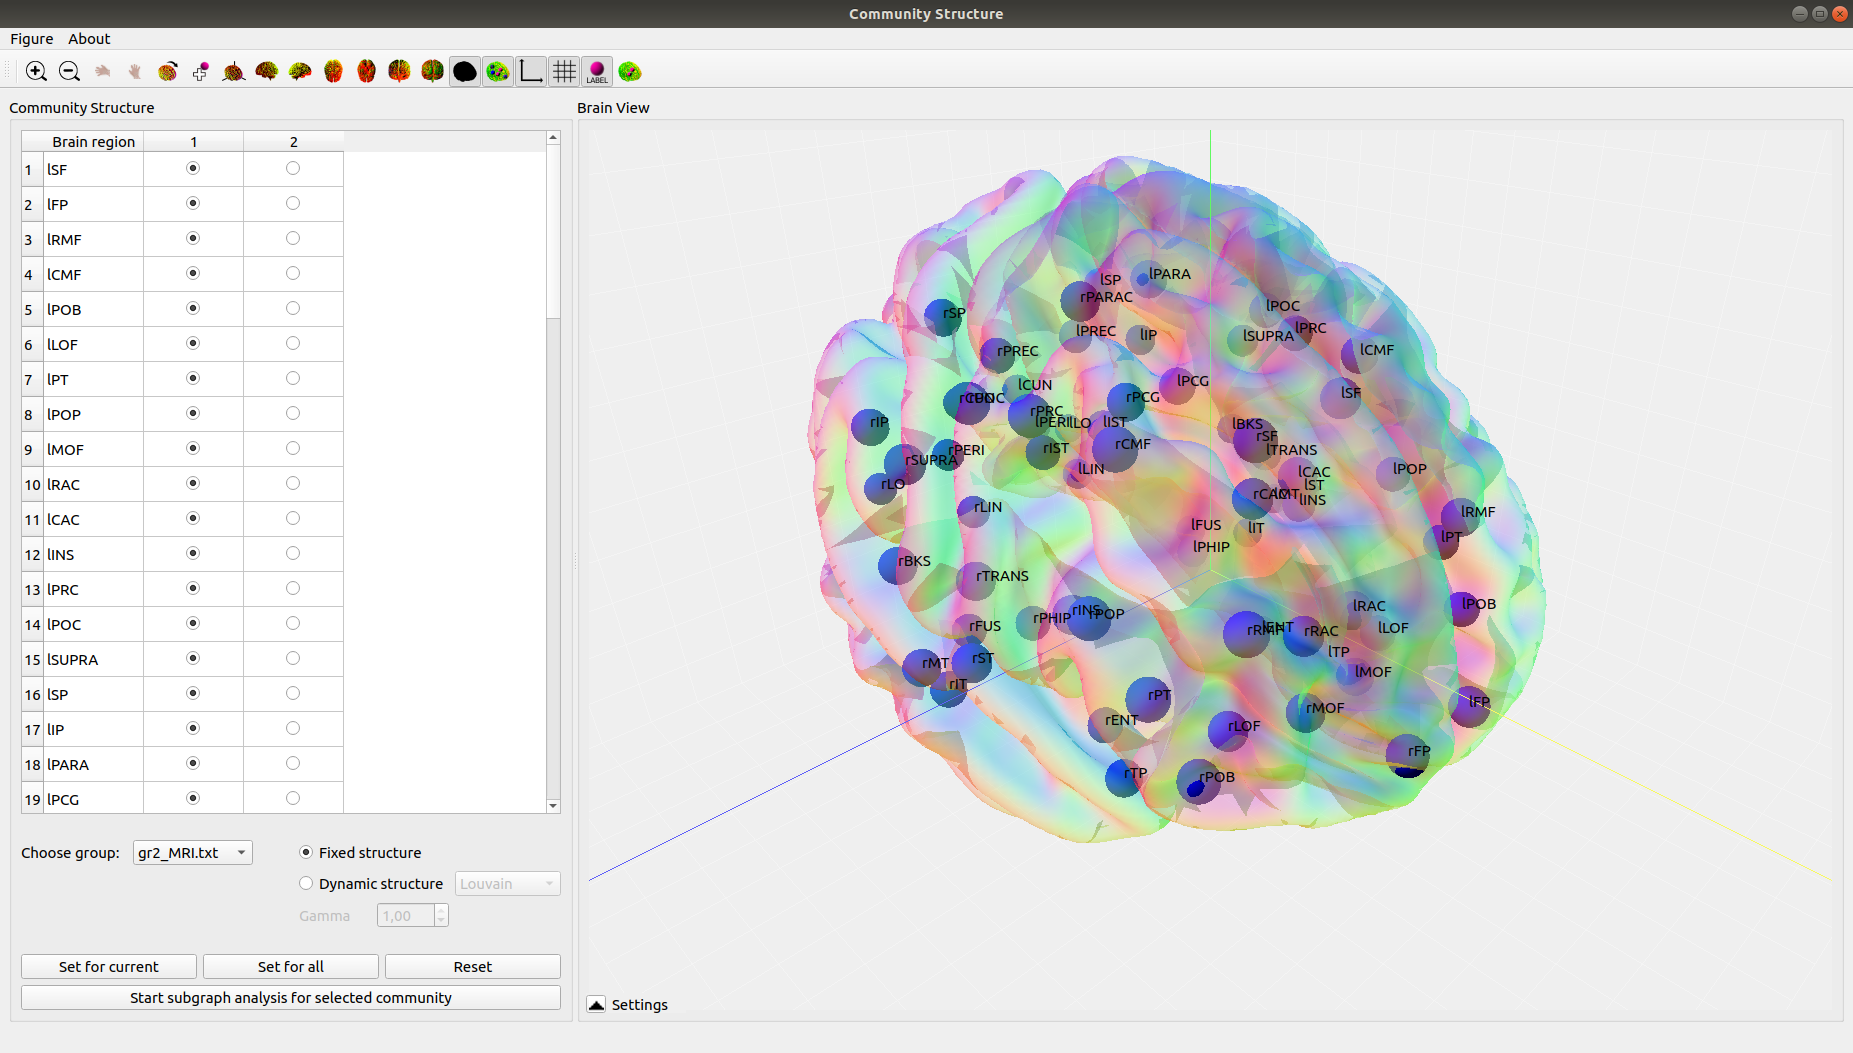
\includegraphics[width=\linewidth]{community_structure.png}
    \caption{The community structure GUI.}
    \label{fig:community}
\end{figure}

\begin{figure}[h]
    \centering
    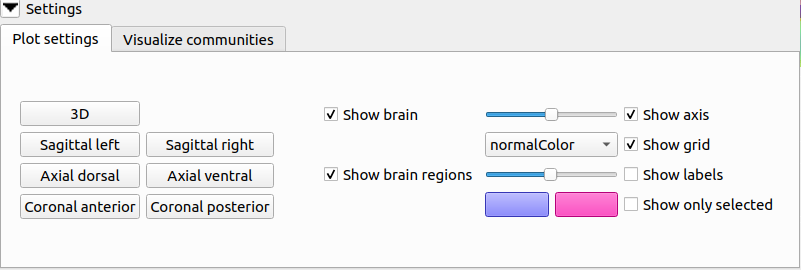
\includegraphics[width=\linewidth]{plot_settings.png}
    \caption{The settings pop-up window in the brain view. Here, the plot settings tab is selected.}
    \label{fig:plot_settings}
\end{figure}

\begin{figure}[h]
    \centering
    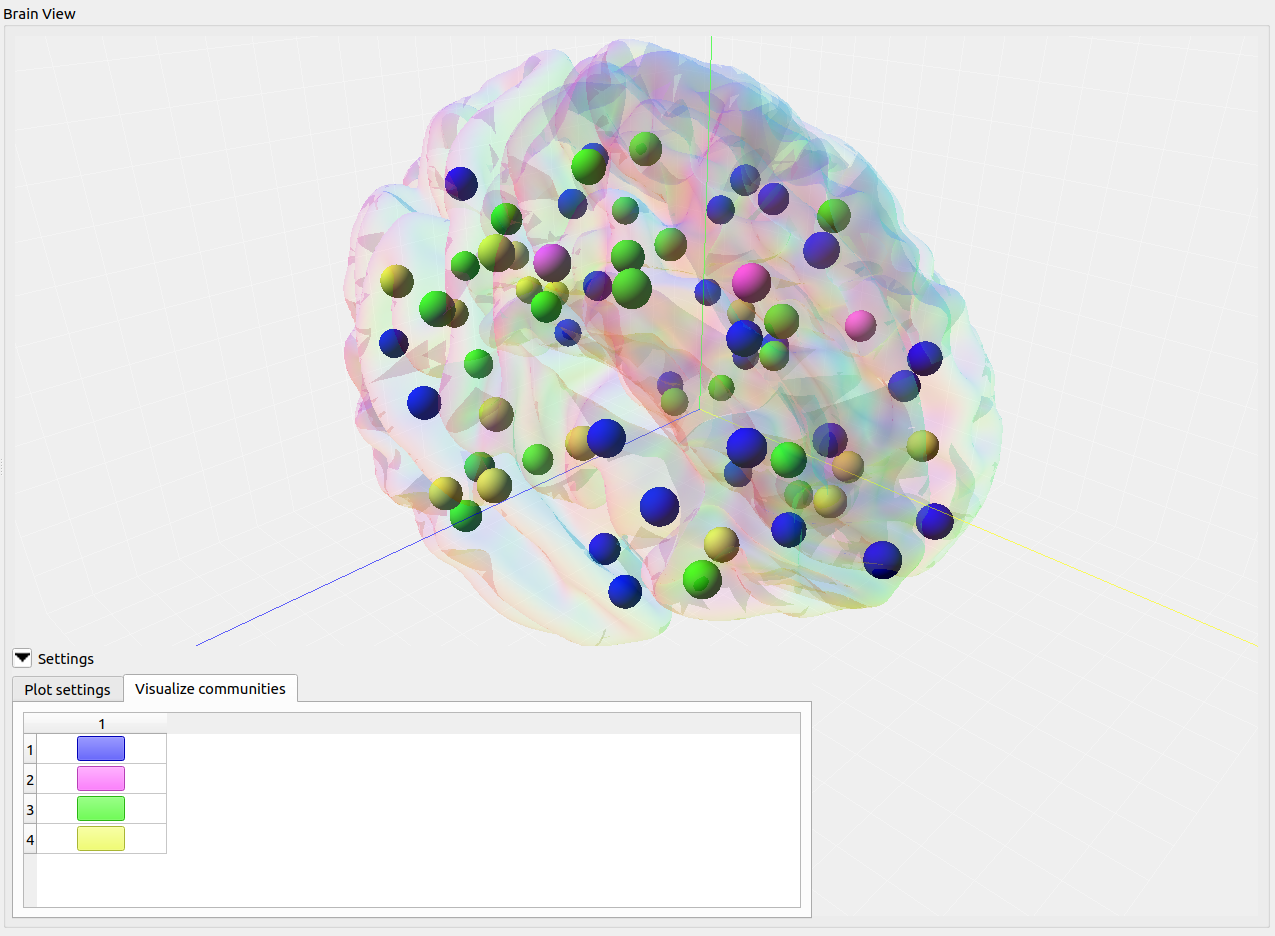
\includegraphics[width=\linewidth]{visualize_communities.png}
    \caption{Using the visualize communities tab, the color of the nodes can be set corresponding to their communities.}
    \label{fig:vis_com}
\end{figure}

The community structure GUI is opened by pressing the 'Edit' button in the Graph Analysis GUI. It can bee seen in \cref{fig:community}. At the top of the window, there is a toolbar which contains buttons that lets the user alter the brain view. For example, you can change the viewpoint, zoom in and out, choose wether to show the brain mesh or not and so on.

If you press the arrow at the bottom left corner of the brain view, a window with two tabs containing more brain view settings appear. This window can be hidden by pressing the arrow again. In the 'Plot settings' tab, see \cref{fig:plot_settings} basic brain view settings can be found. In the 'Visualize communities' tab, see \cref{fig:vis_com}, colors for each community can be defined by pressing on the colored buttons. Note that this tab has to be selected to visualize the communities. 

To edit the communities, use the tools to the bottom left in \cref{fig:community}. Start by selecting what group you want to define the community structure for. Next, choose if you want to use a fixed or a dynamic structure. Here, the fixed structure corresponds to a structure that can be altered manually by the user. A dynamic structure means that the communities are computed according to the selected algorithm and gamma value. Currently, only the Louvain algorithm is implemented. Next, the user can save the community structure displayed in the table. You can either set this structure for the current group, by clicking the button 'Set for current', or you can set it for all group by clicking the button 'Set for all'. If you click 'Reset', the table shows the latest saved community structure for the current group. Note that in order to visualize the communities in the brain view, you have to save them first.

Since this is implemented slightly different than in Braph 1.0, we would like your input on our approach. The reason we did it this way is that we wanted to give more flexibility to the user. For example, you can now use a manually defined community structure for one group and a dynamically computed structure for another group. On the downside, this means that we have to save a community structure for each group in memory. This will be a matrix of size nodes*groups.

The subgraph analysis can be opened from this window, by selecting a column that includes the nodes that you want to use in the subgraph and then pressing 'Start subgraph analysis for selected community'.

\subsubsection{Start Analysis}

\begin{figure}[h]
    \centering
    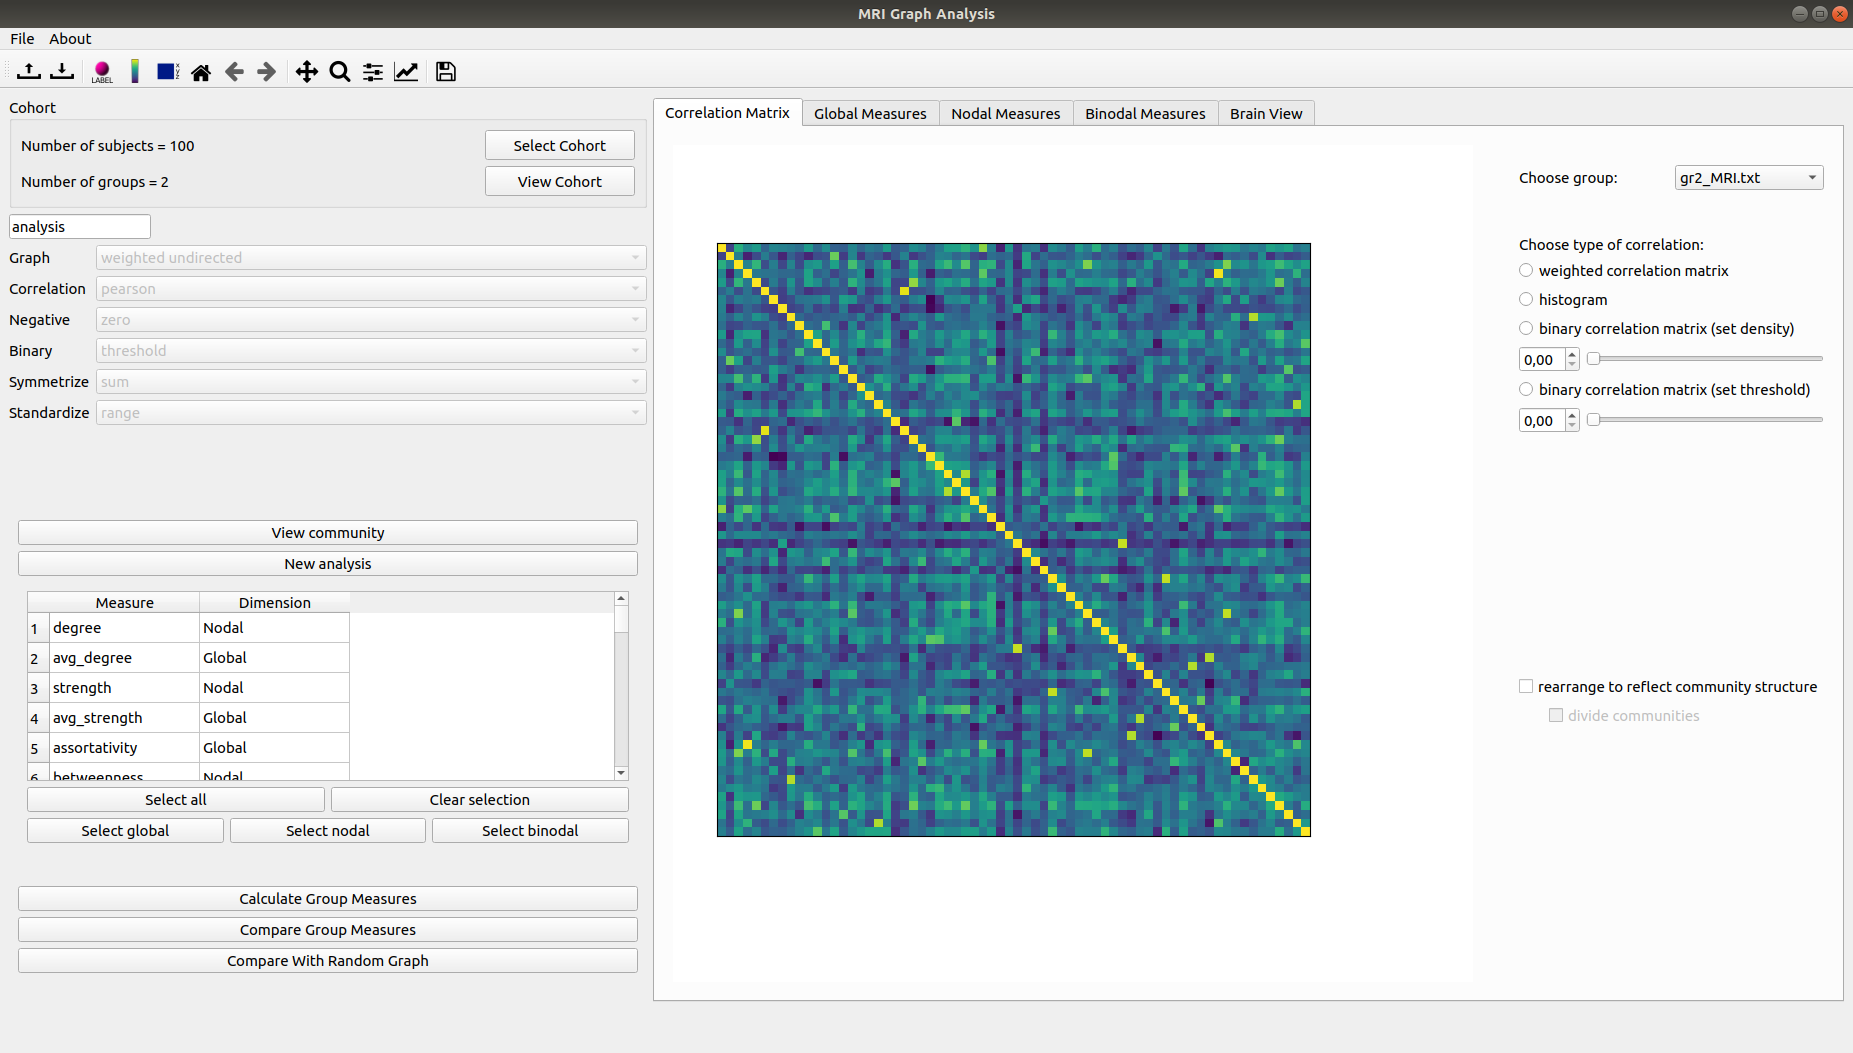
\includegraphics[width=\linewidth]{start_analysis.png}
    \caption{The graph analysis GUI after the start analysis button has been pressed. The graph settings and the community structure is fixed, and additional tabs behind the correlation matrix can be selected. The corresponding view in Braph 1.0 was a new window.}
    \label{fig:start_analysis}
\end{figure}

If you press the 'Start analysis' button in the Graph Analysis GUI, you lock the graph settings and community structure, see \cref{fig:start_analysis}. In Braph 1.0 this opened a new window, but we have chosen to alter the existing window instead, since they are so similar. 

The table of measures don't have a column of descriptions here. Instead, if you hold a cursor over the name of a measure, a desciption of it appears. 

The random comparison is not yet implemented. We are still working on the algorithm for randomization of graphs, and are also waiting to see how you will implement the random caomparison (refering to email conversation).

In the tabs Global, Nodal and Binodal measures, measures and comparisons that are already computed can be seen. These tables and the settings in them are similar to Braph 1.0. The binodal tab is added, and works in the same way as the nodal one, with an additional brain region selection. The data in these tables can be exported as .txt or as .xlsx files. The data in the exported files will be exactely the rows and columns that are displayed in the table. An idea that we have for the future is that you should be able to export all computed measures/comparisons at once here, and not only the ones that are currently displayed in the tables. Perhaps you know best what kind of export alternatives that could be useful here?

In the last tab, different visulizations can be made. Like before, press the arrow to see the settings. The 'Plot settings' tab is identical to before. In the next tab, the graph can be visualized. Hopefully, the settings here are self explanatory. Unfortunately, this is a bit slow for weighted graphs and graphs with high density.

In the tabs 'Visualize measures' and 'Visualize comparisons', nodal measures and comparisons can be visualized. Only measures that are already computed can be selected here. The user can select to visualize the values by size and/or colors of the brain regions. See figures.


\section{fMRI}

\subsection{Graph Analysis fMRI}

\end{document}
